\documentclass[titlepage]{article}
\usepackage[hidelinks]{hyperref}
\usepackage{enumitem}
\usepackage{listings}
\usepackage{xcolor}
\usepackage{forest}
\usepackage{tikz}
\usepackage[T1]{fontenc}



\title{
Homework 1 (Chapter 3) - Due 17th Sep, 2017\\
\begin{large}
Data Structures and Algorithm Analysis in C++
\end{large}
}
\author{Kingsley}
\date{\today}



\usetikzlibrary{matrix,arrows,fit}
\forestset{
	cust-forest/.style={
		for tree={
			circle, draw,
			every node/.style={
				circle, draw,
				inner sep=0pt,
				text width=6mm,
				align=center
			}
		}
	}
}



\begin{document}
\maketitle

\clearpage
\tableofcontents
\clearpage

\section{Basics}
\subsection{Enumerate with alphabet}
\begin{enumerate}[label=(\alph*)]
\item $\Theta(n)$
\item $\Theta(n\log n)$
\item $\Theta(n^2)$
\end{enumerate}

\subsection{inline code}
Inline code example A: \lstinline{for (int i = 0; i < n; i++)}

\lstset{language=C++,keywordstyle={\bfseries \color{orange}}}
Inline code example B: \lstinline{for (int i = 0; i < n; i++)}

Inline code example C: \texttt{for (int i = 0; i < n; i++)}\\

\subsection{code block}
Code block example:

\lstset{
	basicstyle=
		\def\fvm@Scale{0.8}
		\fontfamily{fvm}\selectfont,
	tabsize=4
}
\begin{lstlisting}
int main()
{
	cout << "Hello, World!" << endl;
	return 0;
}
\end{lstlisting}

\LaTeX code example:
\begin{verbatim}
\begin{enumerate}
\item $\Theta(n)$
\item $\Theta(n\log n)$
\item $\Theta(n^2)$
\end{enumerate}
\end{verbatim}

\section{Trees}
\subsection{Binary Tree}

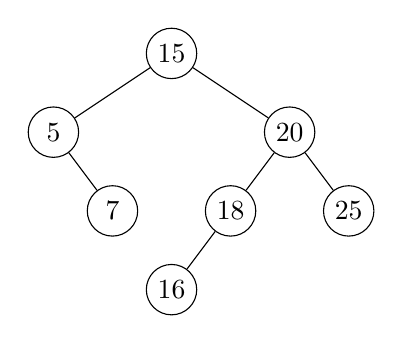
\begin{tikzpicture}[
	every node/.style={
		circle, draw,
		inner sep=0pt,
		text width=6mm,
		align=center
	},
	level distance=10mm,
	level 1/.style={sibling distance=30mm},
	level 2/.style={sibling distance=15mm}
]
\node{$15$}
child { node{$5$}
	child[missing]
	child { node{$7$} }
}
child { node{$20$}
	child { node{$18$}
		child { node{$16$} }
		child[missing]
	}
	child { node{$25$} }
};
\end{tikzpicture}

\subsection{Normal Tree}

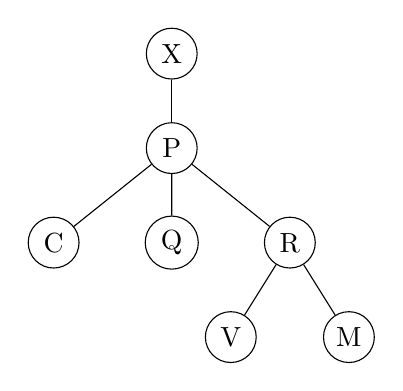
\begin{tikzpicture}[
	every node/.style={
		circle, draw,
		inner sep=0pt,
		text width=6mm,
		align=center
	},
	level distance=1.2cm
]
\node{X}
child { node{P}
	child { node{C} }
	child { node{Q} }
	child { node{R}
		child { node{V} }
		child { node{M} }
	}
};
\end{tikzpicture}

\begin{forest} cust-forest
[, phantom, s sep = 1cm
	[1
		[2[3]]
		[4[5]]
		[6]
	]
]
\end{forest}

\subsection{Forest}

\begin{forest} cust-forest
[, phantom, s sep = 1cm
[A
	[B [C] [D[E]] [F]]
	[G]]
[H
	[I]
	[J [K [L]]
	[M [N] [O]]]]
[P
	[Q] [R [S] [T]] [U] [V [W [X]] [Y]] [Z]]
]
\end{forest}

\leavevmode\vadjust{\vspace{-\baselineskip}}\newline
\begin{center}
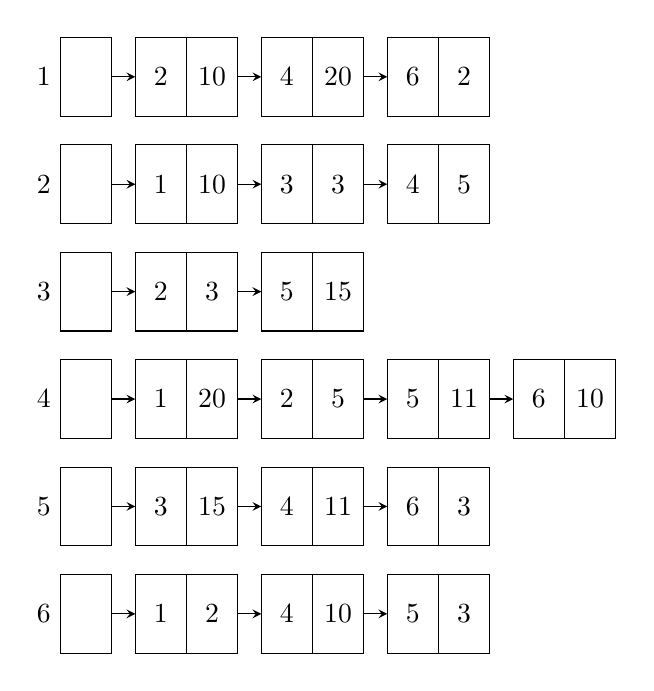
\begin{tikzpicture}[
	circarrow/.style={
		*->, shorten <=-2pt
	}, >=stealth
]
\matrix (M)
[
	matrix of nodes,
	column sep=-\pgflinewidth,
	row sep=3.5mm,
	nodes in empty cells,
	nodes= {
		draw, minimum width=.65cm, outer sep=0pt,
		minimum height=1.0cm, anchor=center
	}
] {
 &[3mm] 2 & 10 &[3mm] 4 & 20 &[3mm] 6 & 2 \\
 & 1 & 10 & 3 & 3 & 4 & 5 \\
 & 2 & 3 & 5 & 15 \\
 & 1 & 20 & 2 & 5 & 5 & 11 &[3mm] 6 & 10 \\
 & 3 & 15 & 4 & 11 & 6 & 3 \\
 & 1 & 2 & 4 & 10 & 5 & 3 \\
};

\foreach \i in {1,2,3,4,5,6} {
	\path (M-\i-1) [late options={label=left:\i}];
	\draw[->] (M-\i-1)--(M-\i-2.west);
	\draw[->] (M-\i-3)--(M-\i-4.west);
}
\draw[->] (M-1-5)--(M-1-6.west);
\draw[->] (M-2-5)--(M-2-6.west);
\draw[->] (M-4-5)--(M-4-6.west);
\draw[->] (M-4-7)--(M-4-8.west);
\draw[->] (M-5-5)--(M-5-6.west);
\draw[->] (M-6-5)--(M-6-6.west);
\end{tikzpicture}
\end{center}

\begin{center}
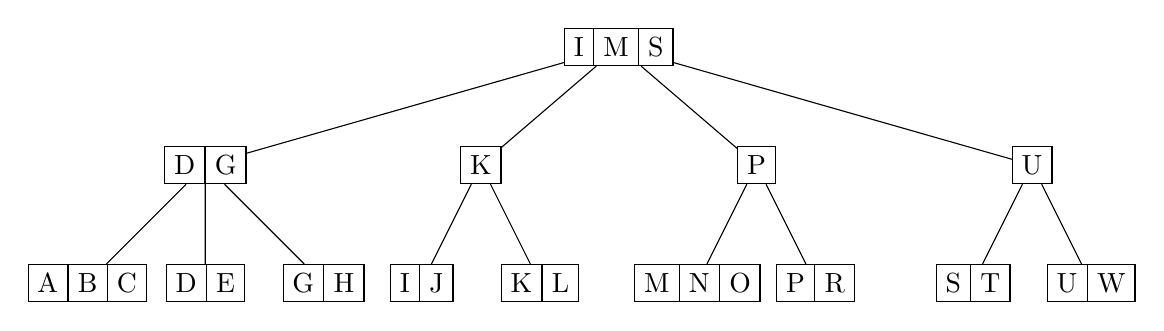
\begin{tikzpicture}
\tikzstyle{bplus}=
[
	draw, rectangle split,
	rectangle split horizontal,
	rectangle split ignore empty parts
]
\tikzstyle{every node}=[bplus]
\tikzstyle{level 1}=[sibling distance=35mm]
\tikzstyle{level 2}=[sibling distance=15mm]

\node {I \nodepart{two} M \nodepart{three} S} [-]
	child {node {D \nodepart{two} G}
		child {node {A \nodepart{two} B \nodepart{three} C}}
		child {node {D \nodepart{two} E}}
		child {node {G \nodepart{two} H}}
	}
	child {node {K}
		child {node {I \nodepart{two} J}}
		child {node {K \nodepart{two} L}}
	}
	child {node {P}
		child {node {M \nodepart{two} N \nodepart{three} O}}
		child {node {P \nodepart{two} R}}
	}
	child {node {U}
		child {node {S \nodepart{two} T}}
		child {node {U \nodepart{two} W}}
	}
;
\end{tikzpicture}
\end{center}

\end{document}
